\section{Application: Principal component analysis}

In this section, we will explore an application of the diagonalization
of symmetric matrices called \textbf{principal component analysis}.
Imagine we are given a collection of data points such as the
following:
\begin{equation}\label{eqn:subspace-fitting}
  \begin{tikzpicture}[baseline=-0.5ex]
    \draw[thin,->] (-4,0) -- (4,0);
    \draw[thin,->] (0,-4) -- (0,4);
    \fill[color=red] (-2.25,-1.21) circle (0.06);
    \fill[color=red] (-1.44,-1.28) circle (0.06);
    \fill[color=red] (2.29,1.82) circle (0.06);
    \fill[color=red] (0.25,0.43) circle (0.06);
    \fill[color=red] (-1.57,-1.07) circle (0.06);
    \fill[color=red] (2.51,2.00) circle (0.06);
    \fill[color=red] (-2.53,-2.34) circle (0.06);
    \fill[color=red] (-3.04,-2.40) circle (0.06);
    \fill[color=red] (0.84,0.36) circle (0.06);
    \fill[color=red] (-3.16,-2.73) circle (0.06);
    \fill[color=red] (-2.02,-1.88) circle (0.06);
    \fill[color=red] (3.06,2.44) circle (0.06);
    \fill[color=red] (-1.40,-1.12) circle (0.06);
    \fill[color=red] (-2.09,-1.34) circle (0.06);
    \fill[color=red] (-1.23,-1.13) circle (0.06);
    \fill[color=red] (0.48,0.06) circle (0.06);
    \fill[color=red] (-1.49,-1.20) circle (0.06);
    \fill[color=red] (0.98,0.75) circle (0.06);
    \fill[color=red] (1.40,0.89) circle (0.06);
    \fill[color=red] (-0.12,0.09) circle (0.06);
    \fill[color=red] (0.88,0.40) circle (0.06);
    \fill[color=red] (-0.38,0.55) circle (0.06);
    \fill[color=red] (0.34,0.46) circle (0.06);
    \fill[color=red] (0.45,0.21) circle (0.06);
    \fill[color=red] (-0.59,-0.63) circle (0.06);
    \fill[color=red] (-0.53,-0.29) circle (0.06);
    \fill[color=red] (2.10,1.35) circle (0.06);
    \fill[color=red] (1.65,1.60) circle (0.06);
    \fill[color=red] (-3.88,-2.83) circle (0.06);
    \fill[color=red] (-0.07,-0.01) circle (0.06);
    \fill[color=red] (-0.37,-0.57) circle (0.06);
    \fill[color=red] (-0.99,-0.75) circle (0.06);
    \fill[color=red] (-2.34,-2.08) circle (0.06);
    \fill[color=red] (3.63,3.15) circle (0.06);
    \fill[color=red] (1.37,0.48) circle (0.06);
    \fill[color=red] (-0.96,-0.74) circle (0.06);
    \fill[color=red] (3.51,2.79) circle (0.06);
    \fill[color=red] (-3.33,-2.72) circle (0.06);
    \fill[color=red] (0.39,0.09) circle (0.06);
    \fill[color=red] (-1.38,-1.17) circle (0.06);
    \fill[color=red] (-0.36,-0.65) circle (0.06);
    \fill[color=red] (1.38,0.66) circle (0.06);
    \fill[color=red] (1.85,1.24) circle (0.06);
    \fill[color=red] (2.35,1.85) circle (0.06);
    \fill[color=red] (0.85,0.25) circle (0.06);
    \fill[color=red] (-0.23,0.19) circle (0.06);
    \fill[color=red] (-0.90,-0.74) circle (0.06);
    \fill[color=red] (2.50,1.31) circle (0.06);
    \fill[color=red] (-0.45,-0.71) circle (0.06);
    \fill[color=red] (0.92,0.56) circle (0.06);
    \fill[color=red] (0.97,1.21) circle (0.06);
    \fill[color=red] (-0.85,-0.74) circle (0.06);
    \fill[color=red] (-0.10,0.13) circle (0.06);
    \fill[color=red] (0.32,0.49) circle (0.06);
    \fill[color=red] (2.58,1.57) circle (0.06);
    \fill[color=red] (-0.59,-0.48) circle (0.06);
    \fill[color=red] (2.28,1.50) circle (0.06);
    \fill[color=red] (1.21,0.94) circle (0.06);
    \fill[color=red] (-0.35,-0.13) circle (0.06);
    \fill[color=red] (-1.53,-1.26) circle (0.06);
    \fill[color=red] (-2.77,-2.14) circle (0.06);
    \fill[color=red] (1.23,1.02) circle (0.06);
    \fill[color=red] (2.61,1.88) circle (0.06);
    \fill[color=red] (-0.04,-0.05) circle (0.06);
    \fill[color=red] (2.09,1.30) circle (0.06);
    \fill[color=red] (2.37,1.52) circle (0.06);
    \fill[color=red] (-2.01,-1.69) circle (0.06);
    \fill[color=red] (0.48,0.72) circle (0.06);
    \fill[color=red] (0.23,0.49) circle (0.06);
    \fill[color=red] (-1.16,-0.95) circle (0.06);
    \fill[color=red] (-0.14,-0.18) circle (0.06);
    \fill[color=red] (-1.57,-1.68) circle (0.06);
    \fill[color=red] (0.39,0.15) circle (0.06);
    \fill[color=red] (-0.24,-0.29) circle (0.06);
  \end{tikzpicture}
\end{equation}
Although these points are spread out in two dimensions, they seem to
be located pretty close to a 1-dimensional subspace. Probably the best
way to interpret this particular data set is to think of the points as
being ``essentially'' on a line, up to some small random errors.

More generally, suppose we are given a collection of data points in
$n$-dimensional space, and we are looking for a $k$-dimensional
subspace that all data points are close to.  This is an important way
to make sense of high-dimensional data. For example, it would be very
difficult to visualize data in a $100$-dimensional space. However, it
we knew that the data points lie very close to a 2-dimensional
subspace, then we could project all of the points to the subspace to
obtain a 2-dimensional image of the data.

To state the problem more precisely, let us introduce the following
notation. If $W$ is a subspace of $\R^n$ and $\vect{v}\in\R^n$ is a
vector, let us write $d(\vect{v},W)$ for the shortest distance from
$\vect{v}$ to $W$ (i.e., the distance from $\vect{v}$ to $W$ along a
line that is perpendicular to $W$). Moreover, if $W$ is a subspace of
$\R^n$ and $\vect{v}_1,\ldots,\vect{v}_m\in\R^n$ are the position
vectors of $m$ points, we define the \textbf{total squared distance}%
\index{distance!total squared distance}%
\index{squared distance}%
\index{total squared distance}%
\index{subspace fitting!total squared distance} of the points to
the subspace to be the quantity
\begin{equation*}
  D(W) = d(\vect{v}_1,W)^2 + \ldots + d(\vect{v}_m,W)^2.
\end{equation*}
Then the problem we would like to solve can be stated as follows:

\begin{problem}{Subspace fitting problem}{subspace-fitting}
  Given vectors $\vect{v}_1,\ldots,\vect{v}_m\in\R^n$ and given an
  integer $k\leq n$, find the $k$-dimensional subspace
  $W\subseteq\R^n$ that minimizes the total squared distance, i.e.,
  such that $D(W)$ is as small as possible.%
  \index{subspace fitting}
\end{problem}

The following proposition gives us a method for solving the subspace
fitting problem. It turns out that the key ingredient in solving this
problem is the diagonalization of symmetric matrices. The method was
discovered by Gale Young%
\index{Young, Gale}%
\index{Gale Young} in 1937.

\begin{proposition}{Solution of the subspace fitting problem}{subspace-fitting}
  Given vectors $\vect{v}_1,\ldots,\vect{v}_m\in\R^n$ and $k\leq n$,
  the optimal solution to the subspace fitting problem can be computed
  as follows:
  \begin{enumerate}
  \item Let $A$ be the $m\times n$-matrix whose rows are
    $\vect{v}_1^T,\ldots,\vect{v}_m^T$. (Or equivalently, $A^T$ is the
    $n\times m$-matrix whose columns are
    $\vect{v}_1,\ldots,\vect{v}_m$.)
  \item Let $B=A^TA$. Then $B$ is a positive semidefinite
    $n\times n$-matrix.
  \item By Proposition~\ref{prop:characterize-positive}, all
    eigenvalues of $B$ are real and non-negative. Let
    $\eigenvar_1,\ldots,\eigenvar_n$ be the eigenvalues of $B$, listed
    according to their multiplicity and in decreasing order, i.e., so
    that $\eigenvar_1\geq\eigenvar_2\geq\ldots\geq\eigenvar_n\geq
    0$. Let $\vect{u}_1,\ldots,\vect{u}_n$ be the corresponding
    eigenvectors.
  \item Then $W=\sspan\set{\vect{u}_1,\ldots,\vect{u}_k}$ is the
    solution to the subspace fitting problem.  Moreover, the total
    squared distance of the points to this subspace is
    \begin{equation*}
      D(W) = \eigenvar_{k+1} + \ldots + \eigenvar_n.
    \end{equation*}
  \end{enumerate}
\end{proposition}

\begin{example}{Subspace fitting in $\R^2$}{subspace-fitting-r2}
  Consider the following collection of points in $\R^2$:
  \begin{equation*}
    \set{
      \begin{mymatrix}{r}  2 \\ -3 \end{mymatrix},
      \begin{mymatrix}{r} -1 \\  0 \end{mymatrix},
      \begin{mymatrix}{r}  2 \\  3 \end{mymatrix},
      \begin{mymatrix}{r} -6 \\ -7 \end{mymatrix},
      \begin{mymatrix}{r}  6 \\ 11 \end{mymatrix},
      \begin{mymatrix}{r}  0 \\ -1 \end{mymatrix},
      \begin{mymatrix}{r}  1 \\  6 \end{mymatrix},
      \begin{mymatrix}{r} -2 \\ -3 \end{mymatrix},
      \begin{mymatrix}{r} -7 \\ -6 \end{mymatrix}
    }.
  \end{equation*}
  Find the 1-dimensional subspace that best approximates this
  collection of points. What is the total squared distance of the
  points to the subspace?
\end{example}

\begin{solution}
  We follow the steps outlined in Proposition~\ref{prop:subspace-fitting}.
  \begin{enumerate}
  \item We have
    \begin{equation*}
      A^T = \begin{mymatrix}{rrrrrrrrr}
        2 & -1 & 2 & -6 & 6 & 0 & 1 & -2 & -7 \\
        -3 & 0 & 3 & -7 & 11 & -1 & 6 & -3 & -6
      \end{mymatrix}.
    \end{equation*}
  \item We calculate
    \begin{equation*}
      B = A^TA = \begin{mymatrix}{rr}
        135 & 162 \\
        162 & 270
      \end{mymatrix}.
    \end{equation*}
  \item The eigenvalues of $B$ are $\eigenvar_1 = 378$ and
    $\eigenvar_2 = 27$, with corresponding eigenvectors
    \begin{equation*}
      \vect{u}_1 = \begin{mymatrix}{r} 2 \\ 3 \end{mymatrix}
      \quad\mbox{and}\quad
      \vect{u}_2 = \begin{mymatrix}{r} 3 \\ -2 \end{mymatrix}.
    \end{equation*}
  \item The desired subspace $W$ is spanned by the eigenvector
    corresponding to the largest eigenvalue, i.e.,
    $W=\sspan\set{\vect{u}_1}$. The total squared distance is
    $\lambda_2 = 27$.
  \end{enumerate}
  The space $W$ is shown in the following illustration, along with the
  original points:
  \begin{equation*}
    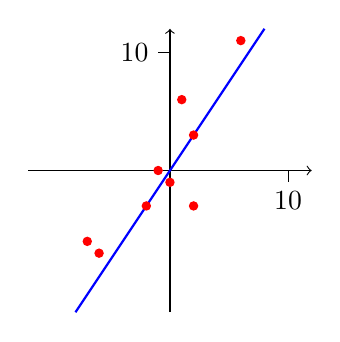
\begin{tikzpicture}[scale=0.15]
      \draw[thin,->] (-12,0) -- (12,0);
      \draw[thin,->] (0,-12) -- (0,12);
      \draw[thin] (0,10) -- (-1,10) node[left] {$10$};
      \draw[thin] (10,0) -- (10,-1) node[below] {$10$};
      \draw[thick,blue] (-8,-12) -- (8,12);
      \fill[color=red] (2,-3) circle (0.4);
      \fill[color=red] (-1, 0) circle (0.4);
      \fill[color=red] (2, 3) circle (0.4);
      \fill[color=red] (-6, -7) circle (0.4);
      \fill[color=red] (6, 11) circle (0.4);
      \fill[color=red] (0, -1) circle (0.4);
      \fill[color=red] (1, 6) circle (0.4);
      \fill[color=red] (-2, -3) circle (0.4);
      \fill[color=red] (-7, -6) circle (0.4);
    \end{tikzpicture}
  \end{equation*}
  Of course, the example was rigged to ensure that the eigenvalues are
  integers. In real life, the entries of $A$ and $B$, as well as the
  eigenvalues and components of the eigenvectors are usually arbitrary
  real numbers.
\end{solution}

\begin{example}{Subspace fitting in $\R^3$}{subspace-fitting-r3}
  Consider the following collection of points in $\R^3$:
  \begin{equation*}
    \set{
      \begin{mymatrix}{r} -7 \\ 4 \\ 5 \end{mymatrix},
      \begin{mymatrix}{r} 0 \\ 3 \\ 3 \end{mymatrix},
      \begin{mymatrix}{r} 2 \\ -5 \\ -4 \end{mymatrix},
      \begin{mymatrix}{r} 10 \\ -4 \\ 1 \end{mymatrix},
      \begin{mymatrix}{r} -2 \\ 5 \\ 4 \end{mymatrix},
      \begin{mymatrix}{r} -8 \\ -1 \\ -5 \end{mymatrix},
      \begin{mymatrix}{r} 5 \\ 4 \\ 2 \end{mymatrix},
      \begin{mymatrix}{r} -6 \\ 9 \\ 6 \end{mymatrix},
      \begin{mymatrix}{r} 9 \\ -6 \\ 3 \end{mymatrix},
      \begin{mymatrix}{r} -2 \\ -7 \\ -8 \end{mymatrix}
    }.
  \end{equation*}
  \begin{enumialphparenastyle}
    \begin{enumerate}
    \item Find the 1-dimensional subspace that best approximates this
      collection of points.
    \item Find the 2-dimensional subspace that best approximates this
      collection of points.
    \item What is the 3-dimensional subspace that best approximates this
      collection of points?
    \end{enumerate}
  \end{enumialphparenastyle}
  In each case, what is the total squared distance of the points to
  the subspace?
\end{example}

\begin{solution}
  Again, we follow the steps from
  Proposition~\ref{prop:subspace-fitting}. We can do the calculations
  for parts (a), (b), and (c) at the same time.
  \begin{enumerate}
  \item We have
    \begin{equation*}
      A^T = \begin{mymatrix}{rrrrrrrrrr}
        -7 & 0 & 2 & 10 & -2 & -8 & 5 & -6 & 9 & -2 \\
        4 & 3 & -5 & -4 & 5 & -1 & 4 & 9 & -6 & -7 \\
        5 & 3 & -4 & 1 & 4 & -5 & 2 & 6 & 3 & -8 \\
      \end{mymatrix}.
    \end{equation*}
  \item We calculate
    \begin{equation*}
      B = A^TA = \begin{mymatrix}{rrr}
        367 & -154 & 16 \\
        -154 & 274 & 170 \\
        16 & 170 & 205 \\
      \end{mymatrix}.
    \end{equation*}
  \item The eigenvalues of $B$ are $\eigenvar_1 = 513$,
    $\eigenvar_2 = 306$, and $\eigenvar_3 = 27$, with corresponding
    eigenvectors
    \begin{equation*}
      \vect{u}_1 = \begin{mymatrix}{r} -2 \\ 2 \\ 1 \end{mymatrix},
      \quad
      \vect{u}_2 = \begin{mymatrix}{r} 2 \\ 1 \\ 2 \end{mymatrix}
      \quad\mbox{and}\quad
      \vect{u}_3 = \begin{mymatrix}{r} -1 \\ -2 \\ 2 \end{mymatrix}.
    \end{equation*}
  \end{enumerate}
  
  For part (a), the desired 1-dimensional subspace is spanned by the
  eigenvector corresponding to the largest eigenvalue, i.e., it is
  $\sspan\set{\vect{u}_1}$. The total squared distance is
  $\eigenvar_2+\eigenvar_3 = 306 + 27 = 333$.

  For part (b), the desired 2-dimensional subspace is spanned by the
  eigenvectors corresponding to the two largest eigenvalues, i.e., it
  is $\sspan\set{\vect{u}_1,\vect{u}_2}$. The total squared distance is
  $\eigenvar_3 = 27$.

  Finally, in part (c), the desired 3-dimensional subspace is spanned
  by all three eigenvectors; it is of course $\R^3$ itself, since it
  is the only 3-dimensional subspace. The total squared distance is
  $0$, since all points lie in the subspace.
\end{solution}

The vectors $\vect{u}_1,\ldots,\vect{u}_n$ that appear in the solution
of the subspace fitting problem are called the \textbf{principal
  components} of the matrix $A$.

\begin{definition}{Principal components}{principal-components}
  Let $A$ be an $m\times n$-matrix. The \textbf{principal components}%
  \index{principal component}%
  \index{component!principal} of $A$ are the (normalized, orthogonal)
  eigenvectors $\vect{u}_1,\ldots,\vect{u}_n$ of the positive
  semidefinite $n\times n$-matrix $A^TA$. They are usually listed in
  order of decreasing eigenvalues.
\end{definition}

The first principal component $\vect{u}_1$ gives the direction in
which the rows of $A$ show the most variability. The second principal
component $\vect{u}_2$ gives the direction in which the rows of $A$
show the most remaining variability that is orthogonal to
$\vect{u}_1$. The third principal component $\vect{u}_3$ gives the
direction of most variability that is orthogonal to $\vect{u}_1$ and
$\vect{u}_2$, and so on.

% ----------------------------------------------------------------------
\subsection*{Subspace fitting vs. curve fitting}

In the particular case where $n=2$ and $k=1$, we are looking for a
1-dimensional subspace, i.e., a line through the origin, which best
fits the given 2-dimensional data, as in the illustration
{\eqref{eqn:subspace-fitting}} above or as in
Example~\ref{exa:subspace-fitting-r2}. On its face, the subspace
fitting problem in this case seems similar to the linear curve fitting
problem we solved in Section~\ref{sec:least-squares}. However, there
is a subtle but important difference: in linear curve fitting, we were
seeking to minimize the distances of the points from the line in the
$y$-direction, whereas in subspace fitting, we are seeking to minimize
the distances of the points from the subspace in the direction
perpendicular to the subspace. The following pair of pictures
illustrates the difference:
\begin{equation*}
  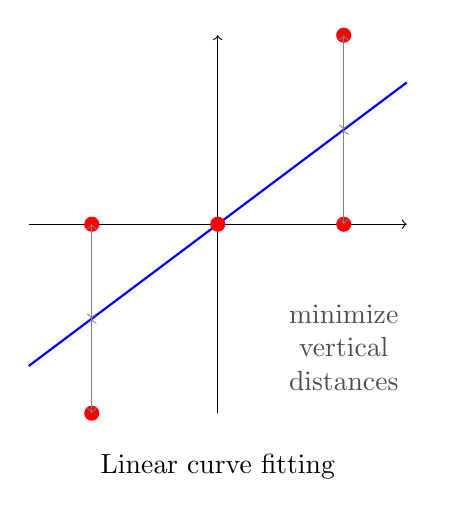
\begin{tikzpicture}[scale=0.8]
    \draw[thin,->] (-3,0) -- (3,0);
    \draw[thin,->] (0,-3) -- (0,3);
    \draw[thick,blue] (-3,-3*0.75) -- (3,3*0.75);
    \fill[color=red] (0,0) circle (0.12);
    \fill[color=red] (2,0) circle (0.12);
    \fill[color=red] (2,3) circle (0.12);
    \fill[color=red] (-2,0) circle (0.12);
    \fill[color=red] (-2,-3) circle (0.12);
    \draw[<->,black!50] (2,0) -- (2,1.5);
    \draw[<->,black!50] (2,3) -- (2,1.5);
    \draw[<->,black!50] (-2,0) -- (-2,-1.5);
    \draw[<->,black!50] (-2,-3) -- (-2,-1.5);
    \path (0,-3.5) node[below] {Linear curve fitting};
    \path[black!70] (2,-2) node {\begin{tabular}{c}minimize\\vertical\\distances\end{tabular}};
  \end{tikzpicture}
  \hspace{1in}
  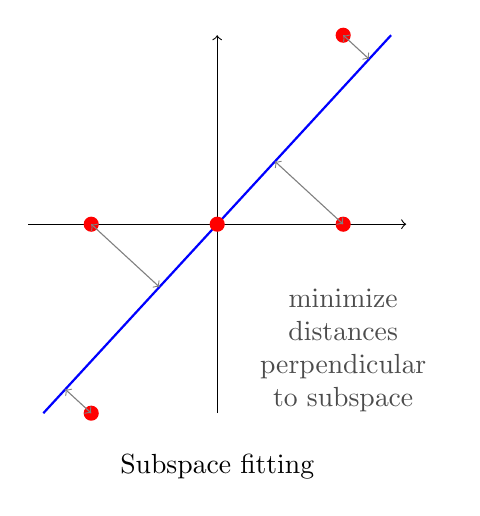
\begin{tikzpicture}[scale=0.8]
    \draw[thin,->] (-3,0) -- (3,0);
    \draw[thin,->] (0,-3) -- (0,3);
    \draw[thick,blue] (-3*0.92,-3) -- (3*0.92, 3);
    \fill[color=red] (0,0) circle (0.12);
    \fill[color=red] (2,0) circle (0.12);
    \fill[color=red] (2,3) circle (0.12);
    \fill[color=red] (-2,0) circle (0.12);
    \fill[color=red] (-2,-3) circle (0.12);
    \draw[<->,black!50] (2,0) -- (0.997*0.92,0.997);
    \draw[<->,black!50] (2,3) -- (2.621*0.92,2.621);
    \draw[<->,black!50] (-2,0) -- (-0.997*0.92,-0.997);
    \draw[<->,black!50] (-2,-3) -- (-2.621*0.92,-2.621);
    \path (0,-3.5) node[below] {Subspace fitting};
    \path[black!70] (2,-2) node {\begin{tabular}{c}minimize\\distances\\perpendicular\\to subspace\end{tabular}};
  \end{tikzpicture}
\end{equation*}

% ----------------------------------------------------------------------
\subsection*{Affine fitting}



% ----------------------------------------------------------------------
\subsection*{Application to U.S. Senate voting data}




% ----------------------------------------------------------------------
\subsection*{CONTINUE HERE}

\begin{equation*}
  \begin{tikzpicture}[scale=0.33]
    \draw[thin,->] (-12,0) -- (12,0);
    \draw[thin,->] (0,-12) -- (0,12);
    \fill[color=red] (-3,-4) circle (0.18);
    \fill[color=red] (6,5) circle (0.18);
    \fill[color=red] (6,11) circle (0.18);
    \fill[color=red] (-6,-5) circle (0.18);
    \fill[color=red] (3,4) circle (0.18);
    \fill[color=red] (-6,-11) circle (0.18);
    \fill[color=red] (0,-3) circle (0.18);
    \fill[color=red] (0,3) circle (0.18);
    \fill[color=red] (0, 0) circle (0.18);
  \end{tikzpicture}
\end{equation*}

\begin{equation*}
  \begin{tikzpicture}[scale=0.5]
    \draw[thin,->] (-4,0) -- (4,0);
    \draw[thin,->] (0,-4) -- (0,4);
    \fill[color=red] (0,1) circle (0.06);
    \fill[color=red] (1,0) circle (0.06);
    \fill[color=red] (0,-1) circle (0.06);
    \fill[color=red] (2, 3) circle (0.06);
    \fill[color=red] (-2, -3) circle (0.06);
    \fill[color=red] (0, 1) circle (0.06);
    \fill[color=red] (1, 0) circle (0.06);
    \fill[color=red] (2, 3) circle (0.06);
    \fill[color=red] (-1, 0) circle (0.06);
  \end{tikzpicture}
\end{equation*}


\begin{equation*}
  \begin{tikzpicture}
    \draw[thin,->] (-4,0) -- (4,0);
    \draw[thin,->] (0,-4) -- (0,4);
    \draw[thick,blue] (-4,-4/1.29) -- (4,4/1.29);
    \fill[color=red] (-2.25,-1.21) circle (0.06);
    \fill[color=red] (-1.44,-1.28) circle (0.06);
    \fill[color=red] (2.29,1.82) circle (0.06);
    \fill[color=red] (0.25,0.43) circle (0.06);
    \fill[color=red] (-1.57,-1.07) circle (0.06);
    \fill[color=red] (2.51,2.00) circle (0.06);
    \fill[color=red] (-2.53,-2.34) circle (0.06);
    \fill[color=red] (-3.04,-2.40) circle (0.06);
    \fill[color=red] (0.84,0.36) circle (0.06);
    \fill[color=red] (-3.16,-2.73) circle (0.06);
    \fill[color=red] (-2.02,-1.88) circle (0.06);
    \fill[color=red] (3.06,2.44) circle (0.06);
    \fill[color=red] (-1.40,-1.12) circle (0.06);
    \fill[color=red] (-2.09,-1.34) circle (0.06);
    \fill[color=red] (-1.23,-1.13) circle (0.06);
    \fill[color=red] (0.48,0.06) circle (0.06);
    \fill[color=red] (-1.49,-1.20) circle (0.06);
    \fill[color=red] (0.98,0.75) circle (0.06);
    \fill[color=red] (1.40,0.89) circle (0.06);
    \fill[color=red] (-0.12,0.09) circle (0.06);
    \fill[color=red] (0.88,0.40) circle (0.06);
    \fill[color=red] (-0.38,0.55) circle (0.06);
    \fill[color=red] (0.34,0.46) circle (0.06);
    \fill[color=red] (0.45,0.21) circle (0.06);
    \fill[color=red] (-0.59,-0.63) circle (0.06);
    \fill[color=red] (-0.53,-0.29) circle (0.06);
    \fill[color=red] (2.10,1.35) circle (0.06);
    \fill[color=red] (1.65,1.60) circle (0.06);
    \fill[color=red] (-3.88,-2.83) circle (0.06);
    \fill[color=red] (-0.07,-0.01) circle (0.06);
    \fill[color=red] (-0.37,-0.57) circle (0.06);
    \fill[color=red] (-0.99,-0.75) circle (0.06);
    \fill[color=red] (-2.34,-2.08) circle (0.06);
    \fill[color=red] (3.63,3.15) circle (0.06);
    \fill[color=red] (1.37,0.48) circle (0.06);
    \fill[color=red] (-0.96,-0.74) circle (0.06);
    \fill[color=red] (3.51,2.79) circle (0.06);
    \fill[color=red] (-3.33,-2.72) circle (0.06);
    \fill[color=red] (0.39,0.09) circle (0.06);
    \fill[color=red] (-1.38,-1.17) circle (0.06);
    \fill[color=red] (-0.36,-0.65) circle (0.06);
    \fill[color=red] (1.38,0.66) circle (0.06);
    \fill[color=red] (1.85,1.24) circle (0.06);
    \fill[color=red] (2.35,1.85) circle (0.06);
    \fill[color=red] (0.85,0.25) circle (0.06);
    \fill[color=red] (-0.23,0.19) circle (0.06);
    \fill[color=red] (-0.90,-0.74) circle (0.06);
    \fill[color=red] (2.50,1.31) circle (0.06);
    \fill[color=red] (-0.45,-0.71) circle (0.06);
    \fill[color=red] (0.92,0.56) circle (0.06);
    \fill[color=red] (0.97,1.21) circle (0.06);
    \fill[color=red] (-0.85,-0.74) circle (0.06);
    \fill[color=red] (-0.10,0.13) circle (0.06);
    \fill[color=red] (0.32,0.49) circle (0.06);
    \fill[color=red] (2.58,1.57) circle (0.06);
    \fill[color=red] (-0.59,-0.48) circle (0.06);
    \fill[color=red] (2.28,1.50) circle (0.06);
    \fill[color=red] (1.21,0.94) circle (0.06);
    \fill[color=red] (-0.35,-0.13) circle (0.06);
    \fill[color=red] (-1.53,-1.26) circle (0.06);
    \fill[color=red] (-2.77,-2.14) circle (0.06);
    \fill[color=red] (1.23,1.02) circle (0.06);
    \fill[color=red] (2.61,1.88) circle (0.06);
    \fill[color=red] (-0.04,-0.05) circle (0.06);
    \fill[color=red] (2.09,1.30) circle (0.06);
    \fill[color=red] (2.37,1.52) circle (0.06);
    \fill[color=red] (-2.01,-1.69) circle (0.06);
    \fill[color=red] (0.48,0.72) circle (0.06);
    \fill[color=red] (0.23,0.49) circle (0.06);
    \fill[color=red] (-1.16,-0.95) circle (0.06);
    \fill[color=red] (-0.14,-0.18) circle (0.06);
    \fill[color=red] (-1.57,-1.68) circle (0.06);
    \fill[color=red] (0.39,0.15) circle (0.06);
    \fill[color=red] (-0.24,-0.29) circle (0.06);
  \end{tikzpicture}
\end{equation*}
